\paragraph{QuizziPedia::Front-End::Views::RegistrationManagementView}
\begin{figure} [ht]
	\centering
	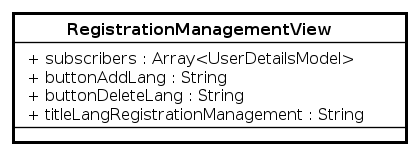
\includegraphics[scale=0.80]{UML/Classi/Front-End/QuizziPedia_Front-end_Views_RegistrationManagementView.png}
	\caption{QuizziPedia::Front-End::Views::RegistrationManagementView}
\end{figure} \FloatBarrier
\begin{itemize}
	\item \textbf{Descrizione}: \textit{view\ped{G}} che permette di visualizzare gli utenti iscritti ad un questionario;
	\item \textbf{Utilizzo}: permette all'utente di visualizzare gli utenti iscritti ad un questionario e, tramite apposita sezione, approvare l'iscrizione;
	\item \textbf{Relazioni con altre classi}:
	\begin{itemize}
		\item \textbf{IN \texttt{RegistrationManagementModelView}}: classe di tipo modelview la cui istanziazione è contenuta all'interno della variabile di ambiente \texttt{\$scope} di \textit{Angular\ped{G}}. All'interno di essa sono presenti le variabili e i metodi necessari per il \textit{Two-Way Data-Binding\ped{G}} tra la \textit{view\ped{G}} \texttt{RegistrationManagementView} e il \textit{controller\ped{G}} \texttt{RegistrationManagementController};
		\item \textbf{IN \texttt{LangModel}}: rappresenta il modello delle informazioni per la giusta traduzione dell'applicazione.
	\end{itemize}
	\item \textbf{Attributi}:
	\begin{itemize}
		\item \texttt{+ subscribers: Array<UserDetailsModel>} \\ \texttt{array} contenete un oggetto per ogni utente iscritto al questionario. L'oggetto sarà composto dai campi \texttt{nome} e \texttt{cognome};
		\item \texttt{+ buttonAddLang: String} \\ Attributo che viene utilizzato per visualizzare la giusta traduzione del bottone di approvazione iscrizione di un utente, in italiano o in inglese;
		\item \texttt{+ buttonDeleteLang: String} \\ Attributo che viene utilizzato per visualizzare la giusta traduzione del bottone di disiscrizione di un utente, in italiano o in inglese;
		\item \texttt{+ titleLangRegistrationManagement: String} \\ Attributo che viene utilizzato per visualizzare la giusta traduzione del titolo della pagina, in italiano o in inglese;		
	\end{itemize}
\end{itemize}